\documentclass{article}

\usepackage{amsmath}
\usepackage{amssymb}
\usepackage{amsfonts}
\usepackage{mathtools}

\usepackage[thmmarks, amsmath]{ntheorem}

\usepackage{graphicx}
\usepackage{float}
\usepackage{tikz-cd}

\usepackage{diffcoeff}
\diffdef{}{op-symbol=\mathrm{d},op-order-sep=0mu}

\usepackage{cancel}
\usepackage{interval}

\usepackage{array}

\usepackage{enumitem}

\setlist[enumerate,1]{label=(\alph*)}

\title{Algebraic Topology Homework 4}
\author{Duarte Maia}
%\date{}

\theoremstyle{plain}
\theorembodyfont{\upshape}
\theoremseparator{.}
\newtheorem{theorem}{Theorem}
\newtheorem{prop}{Prop}
\renewtheorem*{prop*}{Prop}
\newtheorem{lemma}{Lemma}
\newtheorem*{ex}{Exercise}

\theoremstyle{nonumberplain}
\theoremheaderfont{\itshape}
\theorembodyfont{\upshape}
\theoremseparator{:}
\theoremsymbol{\ensuremath{\blacksquare}}
\newtheorem{proof}{Proof}
\newtheorem{sol}{Solution}

\theoremsymbol{\text{\textit{(End proof of lemma)}}}
\newtheorem{lemmaproof}{Proof of lemma}

\newcommand{\R}{\mathbb{R}}
\newcommand{\C}{\mathbb{C}}
\newcommand{\Z}{\mathbb{Z}}
\newcommand{\Q}{\mathbb{Q}}

\newcommand{\RP}{\mathbb{RP}}

\newcommand{\kk}{\Bbbk}

\newcommand{\PP}{\mathbb{P}}
\newcommand{\FF}{\mathcal{F}}

\newcommand{\I}{\mathrm{i}}
\newcommand{\e}{\mathrm{e}}

\newcommand{\id}{\mathrm{id}}

\newcommand{\conj}[1]{\overline{#1}}
\newcommand{\close}[1]{\overline{#1}}

\DeclareMathOperator{\inte}{int}
\DeclareMathOperator{\codim}{codim}
\newcommand{\grad}{\nabla}


\DeclareMathOperator{\spec}{spec}

\DeclarePairedDelimiter{\abs}{\lvert}{\rvert}
\DeclarePairedDelimiter{\norm}{\lvert}{\rvert}
\DeclarePairedDelimiter{\Norm}{\lVert}{\rVert}
\DeclarePairedDelimiter{\braket}{\langle}{\rangle}


\begin{document}
\maketitle

\begin{ex}[2.1:17]
\leavevmode
\begin{enumerate}
\item Compute $H_n(X,A)$ when $X = S^2$ or $T^2$ and $A$ is a finite set of points in $X$.
\item Compute $H_n(X,A)$ and $H_n(X,B)$ where $X$ is a closed surface of genus two and $A$ and $B$ are the circles shown in Hatcher.
\end{enumerate}
\end{ex}

\begin{sol}
\leavevmode
\begin{enumerate}
\item Let us look at the long exact sequence. In both cases, the homology of $X$ is null from index $2$ onwards, and the homology of $A$ is null after index $0$, so it is trivial to see that $H_n(X,A)$ is null for $n > 2$. Therefore, we represent only the long exact sequence until $n = 2$:
\begin{equation}
\begin{aligned}
\cdots \to H_3(X,A) &\to \tilde H_2(A) \to \tilde H_2(X) \to H_2(X,A) \to\\
&\to \tilde H_1(A) \to \tilde H_1(X) \to H_1(X,A) \to\\
&\to \tilde H_0(A) \to \tilde H_0(X) \to H_0(X,A) \to 0
\end{aligned}
\end{equation}
and applying elementary simplifications we obtain the following (simplified) sequence
\begin{equation}
\begin{aligned}
\cdots \to 0 &\to 0 \to \tilde H_2(X) \to H_2(X,A) \to\\
&\to 0 \to \tilde H_1(X) \to H_1(X,A) \to\\
&\to \Z^{n-1} \to 0 \to H_0(X,A) \to 0
\end{aligned}
\end{equation}
where $n = \# A$.

Therefore, we conclude that $H_2(X,A) \cong H_2(X) \cong \Z$, as well as $H_0(X,A) = 0$. Moreover, we have that the following sequence is exact
\begin{equation}
0 \to H_1(X) \to H_1(X,A) \to \Z^{n-1} \to 0.
\end{equation}

Now, in the case $X = S^2$ we have $H_1(X) = 0$ (because $\pi_1(X) = 0$) and hence $H_1(X,A) \cong \Z^{n-1}$ in this case. On the other hand, if $X = T^2$ we have $H_1(X) \cong \Z^2$ and the computation of $H_1(X,A)$ becomes less obvious.

The exact sequence now becomes
\begin{equation}
0 \to \Z^2 \to H_1(X,A) \to \Z^{n-1} \to 0.
\end{equation}

Okay well, to compute $H_1(X,A)$ I'll use the following trick. Since $(X,A)$ is a good pair (any finite subset of a topological manifold is good, kind of trivially) the relative homology coincides with the reduced homology of $X/A$. Now, in a nice enough space (as is the case here), identifying two points is homotopically equivalent to wedging a copy of $S^1$ to the space, and arguing inductively we see that $X/A$ is equivalent to the torus wedged with $n-1$ copies of $S^1$. Now, the reduced homology $\tilde H_1(X/A)$ is additive under wedges (assuming the basepoint is nicely included in the spaces being wedged, which is the case here) so we see that $\tilde H_1(X/A) \cong \Z^2 \oplus \Z^{n-1}$, the first term coming from the torus and the second from the $n-1$ circles. This concludes the computation of $H_*(X,A)$.

\item Well, $A$ and $B$ are good subsets of $X$, so the relative homologies coincide with the reduced homologies of $X/A$.

Now, $X/A$ is the wedge of two tori, and the reduced homology is additive wrt the wedge sum (assuming that the basepoints have contractible neighbourhoods, as is the case). Therefore, the relative homology $H_n(X,A)$ is simply the squares (as groups) of the reduced homology of the the torus, which is known to be $0$, $\Z^2$, $\Z$ in degrees $0$, $1$, $2$ respectively and null in higher degrees. Thus, the relative homologies $H_n(X,A)$ are given by $0$, $\Z^4$, $\Z^2$, and then zeroes.

On the other hand, $X/B$ is homotopically equivalent to a torus wedged with a circle, so by the same argument the relative homologies $H_n(X,B)$ are given by $0$, $\Z^3$, $\Z$, and then zeroes.
\end{enumerate}
\end{sol}

\begin{ex}[2.1:29]
Show that $T^2$ and $S^1 \vee S^1 \vee S^2$ have isomorphic homology groups in all dimensions but their universal covering spaces do not.
\end{ex}

\begin{sol}
Okay well, the isomorphic homology groups part is easy. First, use reduced homology because that's equivalent, and then use the fact that reduced homology is additive under nice wedges. Indeed, this trick works to make spaces whose homology groups are any finite sequence of finitely generated free groups, by just wedging an $S^n$ for each generator in dimension $n$.

Now, the universal cover of $T^2$ is just $\R^2$, whose reduced homology groups are all trivial. On the other hand, $S^1 \vee S^1 \vee S^2$ has as universal cover the thing in the following figure, which is homotopically equivalent to a wedge of countably many spheres, which has nontrivial second homotopy group (blah blah reduced homology wedges, it's $\Z^{\oplus \infty}$).
\begin{figure}[H]
\centering
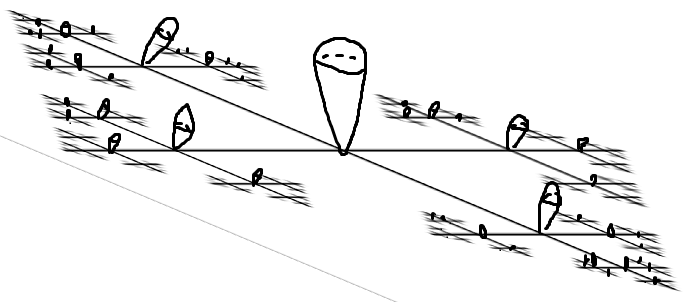
\includegraphics{perspective}
\caption{Universal cover of $S^1 \vee S^1 \vee S^2$.}
\end{figure}

(End of solution)
\end{sol}

\begin{ex}[2.1:31]
Give an example of the five lemma where all but the middle map are zero.
\end{ex}

\begin{sol}
% https://tikzcd.yichuanshen.de/#N4Igdg9gJgpgziAXAbVABwnAlgFyxMJZABgBpiBdUkANwEMAbAVxiRGJAF9T1Nd9CKAIzkqtRizYduvbHgJEATKOr1mrRCAA6WgFpceIDHIFEAzCvHq2O-TKN95g5ABZLayZumHj-BSjIhMQ8NdgNZP2cRINUJUNtwhxN-ZGUYq09tPUTfJ3NSdJCpHMdTFDdCuOLOMRgoAHN4IlAAMwAnCABbJDIQHAgkAFZ7dq6e6n6kIRGO7sRBiYHEADYZscQRPqXVw1G5zcnERTW55S2kMxOLxaQXK8Q3c8QATnuLJ4AOe7PDgHZ7343RBfXazJDLIH-CicIA
\leavevmode
\begin{figure}[H]
\centering
\begin{tikzcd}
0 \arrow[d] \arrow[r] & 0 \arrow[d] \arrow[r] & \Z \arrow[r] \arrow[d] & \Z \arrow[r] \arrow[d] & 0 \arrow[d] \\
0 \arrow[r]           & \Z \arrow[r]          & \Z \arrow[r]           & 0                      \arrow[r] & 0          
\end{tikzcd}
\end{figure}

In the previous picture, all arrows $\Z \to \Z$ are the identity. All others are obviously zero.
\end{sol}

\begin{ex}[2.2:2]
Given an automorphism of an even-dimensional sphere, show that there exists some point $x$ which is taken to itself or its antipodal.

Deduce that every automorphism of an even-dimensional real projective space has a fixed point. Show that this is not true of odd-dimensional real projective spaces.
\end{ex}

\begin{sol}
Suppose by contradiction that there exists some automorphism $f$ of an even-dimensional sphere, such that $f(x)$ is never $x$ or $-x$. In particular, $f$ has no fixed points, and therfore, by property (g) of the degree (page 134 in Hatcher) has degree $-1$. On the other hand, $-f$ also has no fixed point, and therefore also has degree $-1$. But also, $-f$ is the composition of $f$ and the antipodal map, which also has degree $-1$, so we reach the contradiction $-1 \times -1 = -1$, whence such a map $f$ cannot exist.

From this we conclude the statement about automorphisms of even-dimensional real projective spaces easily, because if $f$ is an automorphism of an even-dimensional projective space then $f \circ \pi$ is a map from $S^{2n}$ to $\R \PP^{2n}$, which lifts to an automorphism $\tilde f$ of $S^{2n}$ because $S^{2n}$ is the universal cover of $\R \PP^{2n}$. Now, for this automorphism there must be some point $x$ such that $\tilde f(x) = \pm x$, and by passing to the quotient we get that $f([x]) = [x]$.

For odd-dimensional real projective spaces, we find a counterexample by building a linear automorphism of $\R^{2n}$ which has no eigenvalues, as it then passes to an automorphism of $\R \PP^{2n-1}$, and the lack of eigenvalues is equivalent to the latter map having no fixed points.

Here are a couple of ways to do it. One way is to just make a block diagonal matrix composed of rotation matrices with angles different from $0^\circ$ and $180^\circ$, as these have no eigenvectors. Another way to do it is to use the concept of companion matrix from algebra, which allows us to make an automorphism of $\R^{2n}$ whose characteristic polynomial is any of our choosing. In particular, we may consider the companion matrix of $x^{2n} + 1$, which has no real roots, and hence its companion matrix has no real eigenvectors.
\end{sol}

\begin{ex}[2.2:8]
Show that the degree of a complex polynomial (in the usual sense) coincides with the degree of its extension to the one-point compactification.
\end{ex}

\begin{sol}
We apply the differential formula for the degree. To this effect, we begin by noting that if $p$ is a polynomial then it has finitely many critical values (because its derivative either has finitely many zeros or $p$ is constant itself), and therefore we may pick some $y$ which is a regular value of $p$. Then, we apply the local formula for the degree of $\hat p$, using this value of $y$.

Now, without loss of generality, suppose that $y = 0$; the rest of the proof will follow even if $y$ is not zero, but is a bit more cumbersome to write. By the differential formula for the degree, we get that the degree of $\hat p$ is equal to the local degree of $p$ at all of its roots. But all of its roots are nondegenerate (because we assumed $y$ was a regular value) and therefore, in a neighborhood of each root, $p$ is a homomorphism. Moreover, because it's a complex polynomial and therefore holomorphic, in a neighborhood of reach root $p$ is an \emph{orientation perserving} homomorphism. As such, each root has local degree equal to $+1$, and so the total degree of $\hat p$ is equal to $(+1) \times \text{\#roots}$, which is precisely the degree of $p$.
\end{sol}

\begin{ex}[2.2:16]
Compute the ranks of the simplicial chain groups and the subgroups of cycles and boundaries. Apply this to show that the $k$-skeleton of $\Delta^n$ has homology groups $\tilde H_i((\Delta^n)^k)$ equal to  $0$ for $i<k$ and free of rank $\binom n {k+1}$ for $i = k$.
\end{ex}

\begin{sol}
(Until the end of the solution, we will be talking about the reduced chain complex.)

Well, a generating $k$-chain of $\Delta^n$ consists of choosing $k+1$ vertices and taking the $k$-simplex generated by them. Therefore, the group of $k$-chains has rank $\binom{n+1}{k+1}$.

Now, among these, the cycles and the boundaries are the same. This is because we know the singular, and hence simplicial, homology of $\Delta^n$ is null because this space is contractible. Therefore, it suffices to compute how many chains are cycles or how many chains are boundaries.

We compute how many cycles there are. We will show that the answer is $\binom{n}{k+1}$, and to do so we show that there is a one-to-one correspondence between $k$-chains of $A = [v_1, \dots, v_n]$ and $k$-cycles of $X = [v_0, \dots, v_n]$.

Given a $k$-cycle of $X$, we define a corresponding $k$-chain of $A$ by projecting onto the component of chains of $A$; in other words, we throw away the generators which have $v_0$ as a vertex.

Given a $k$-chain $c$ of $A$, we define a corresponding $k$-cycle of $X$ as follows. First, consider $\partial c$, which is a sum of $k-1$-symplices of $A$. To these, we add the vertex $v_0$ at the start, to yield a sum $S$ of $k$-symplices of $X$. Then, to to the $k$-chain $c$ we assign the $k$-cycle $c + S$.

It is easy to verify that these two maps are both group homomorphisms and are inverses of each other, and therefore the group $k$-cycles of $X$ is isomorphic to the group of $k$-chains of $A$, which we already know is free of rank $\binom{n}{k+1}$.

\smallskip

Now we can easily compute the reduced homology of the $k$-skeleton of $\Delta^n$. Indeed, it coincides with the simplicial homology of $\Delta^n$ at degrees $i < k$, and at $i = k$ it coincides with the group of $k$-cycles of $\Delta^n$, which as we just saw is free of rank $\binom n {k+1}$.
\end{sol}

\end{document}